\chapter{Solutions and Implementation}

This chapter presents the design and implementation of \textit{TextLens}, an offline, real-time scene text translation application for Android. Unlike a client--server architecture, the system is implemented primarily as an \textbf{on-device pipeline}, where camera capture, text recognition, translation, and scene text replacement are performed locally on the mobile device. This design reduces network dependency, improves privacy, and supports real-time use in environments with limited or no internet access.

\section{System Implementation}
The diagram below shows the high level implement of how the entire system works.

\begin{figure}[h]
\centering
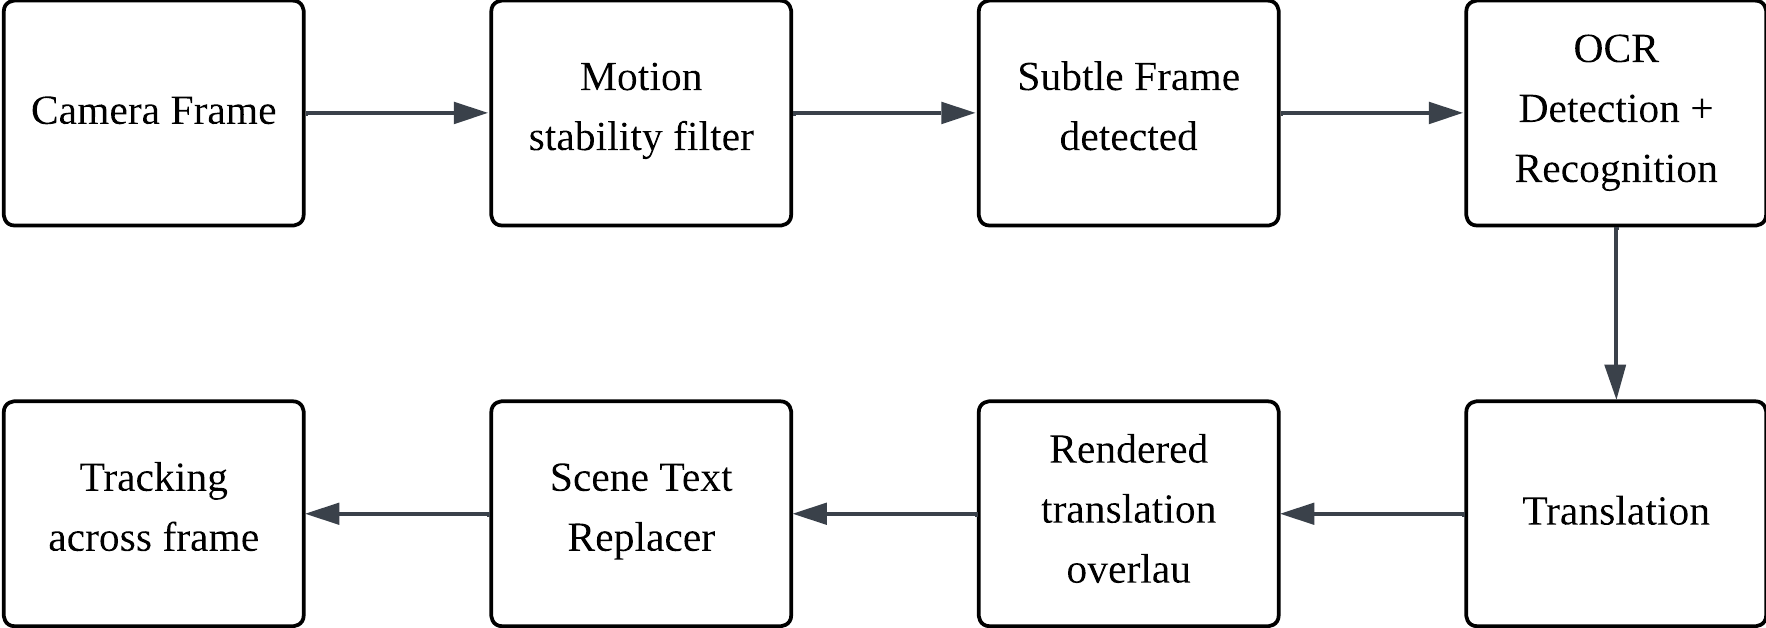
\includegraphics[width=0.85\linewidth]{fig/pipeline.png}
\caption{TextLens processing pipeline for real-time scene text translation.}
\label{fig:pipeline}
\end{figure}

\subsection{Frontend and On-Device Processing Implementation}
The diagram below shows an overview of how the frontend and on-device processing is like:

\begin{figure}[H]
    \centering
    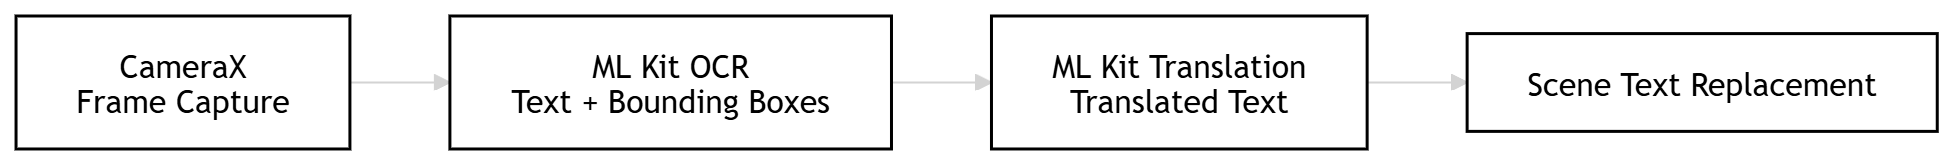
\includegraphics[width=\linewidth]{fig/frontendflow.png}
    \caption{Flowchart showing how the frontend and On-Device processing work}
    \label{fig:textlens-camera}
\end{figure}

The core implementation of TextLens is built as an on-device Android pipeline using Kotlin. The application captures live camera frames using \textbf{CameraX}, performs text recognition using \textbf{ML Kit OCR}, translates the detected text using \textbf{ML Kit's on-device translation}, and finally redraws the translated text back into the image using a custom \textbf{scene text replacement} module. Unlike a simple overlay-based approach, the system attempts to preserve the original appearance of the scene by removing the original text region and rendering the translated content directly within the same area.

Text recognition is performed using ML Kit OCR, which detects text lines and returns both the recognized text and its associated spatial information, including bounding boxes and corner points. These outputs are essential because they define where the translated text should later be inserted. The OCR results are stored at runtime and passed into the later stages of the processing pipeline.

After OCR, the recognized text is translated using ML Kit's on-device translation library. Since the translation models are stored locally on the device, this stage supports the project's offline requirement and avoids dependence on continuous internet connectivity.

\subsection{Scene Text Replacement}

An important component of the implementation is the \texttt{SceneTextReplacer} module, which replaces detected source text with translated text while preserving the visual appearance of the scene. The module is implemented as a dedicated class that receives three inputs: the current image frame, OCR detection results, and the corresponding translated strings. Its primary function is to remove the detected text and render the translated output so that it appears naturally integrated into the image.

The process begins by validating the input frame and converting it into a consistent \textbf{BGR OpenCV Mat} format. Since camera frames may arrive in different channel formats such as grayscale, RGB, or RGBA, they are first normalized to ensure compatibility with subsequent image processing steps. A copy of the original frame is also preserved so that colour information from the original text regions can later be used during rendering.

The module then filters the OCR results to construct a list of valid text items. Each detection must contain both a valid bounding region and a corresponding translated string. Detections with empty translations or invalid geometry are discarded to ensure that only meaningful regions are processed.

To remove the original text, the system performs an \textbf{inpainting step}. A binary mask is generated for all valid text regions using either OCR polygon points or axis-aligned bounding boxes. The mask is expanded using morphological dilation to cover character edges and prevent residual artifacts. OpenCV’s \texttt{Photo.inpaint()} function is then applied using the \textbf{Telea algorithm} to reconstruct the background beneath the removed text.

After inpainting, the system estimates suitable rendering colours for the translated text. The background colour is sampled from the inpainted frame, while the original text colour is estimated from the preserved copy of the original image. Pixels within the region are sampled with an adaptive step size and separated into dark and light groups based on luminance to infer likely background and foreground colours.

The translated text is then rendered using the Android \textbf{Canvas} API. The OpenCV frame is temporarily converted to a bitmap, and a reusable buffer is maintained to avoid repeated memory allocation during continuous processing. Text size is determined from the bounding box height and adjusted if the translated string exceeds the available width. An additional scaling factor ensures that the rendered text fits comfortably within the region.

To maintain the original scene layout, the module also estimates the \textbf{text orientation}. The rotation angle is derived from OCR corner points representing the top edge of the detected text. If the angle is small, it is approximated as zero; otherwise, the canvas is rotated about the region centre before rendering the text. This allows translated text to follow the original orientation of the detected words.

Finally, the rendered bitmap is converted back into an OpenCV Mat so that the processed frame can continue through the application pipeline. The result is an image frame in which the original text has been removed and replaced with translated text that visually aligns with the surrounding scene.

\begin{figure}[H]
    \centering
    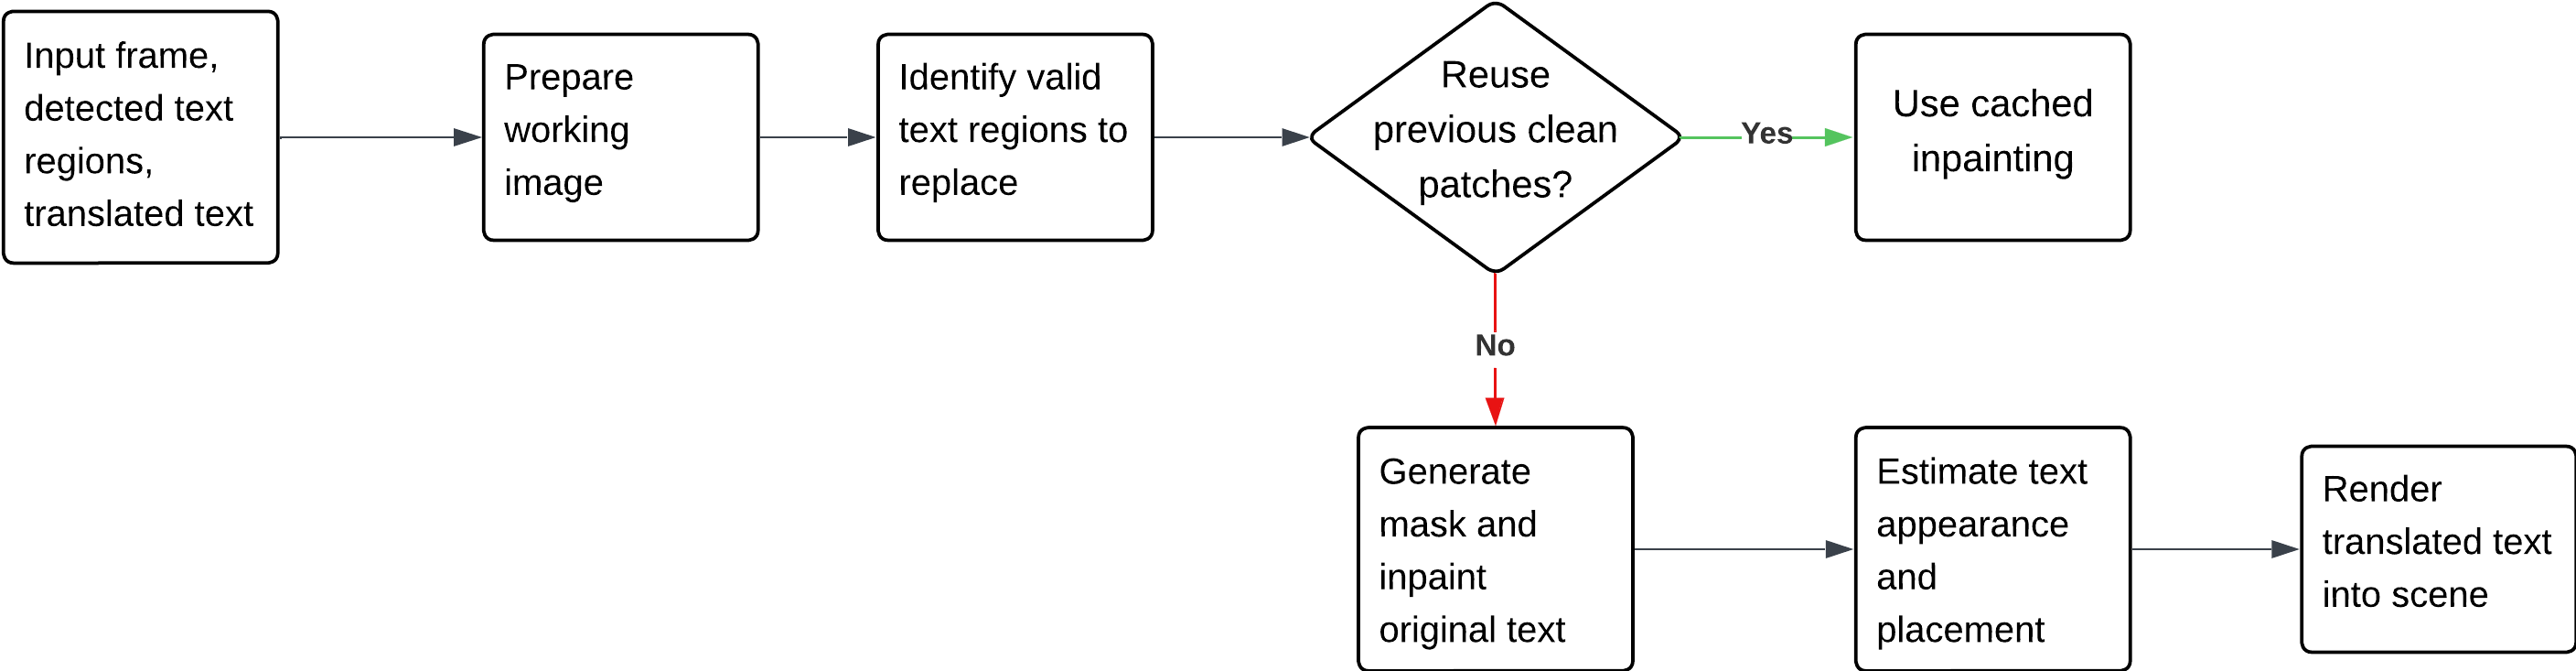
\includegraphics[width=\linewidth]{fig/scenetext.png}
    \caption{Implementation of the scene text replacement pipeline}
    \label{fig:textlens-scene-replace}
\end{figure}

\subsection{Tracking Mechanism}

To avoid performing OCR on every camera frame, the system uses a tracking mechanism to maintain the positions of previously detected text regions. After a stable frame is identified and OCR has been executed, the resulting text bounding boxes are stored as a reference. These regions are then tracked across subsequent frames so that the translated text remains aligned with the scene during small camera movements.

For each new frame, motion between the current frame and the reference frame is estimated using feature-based tracking. Visual feature points are extracted from the areas surrounding the detected text regions, and their displacement is measured across frames. From these correspondences, a geometric transformation is computed and applied to the stored bounding boxes to update their positions without requiring another OCR pass.

If camera motion becomes excessive or the transformation becomes unreliable, the tracking state is discarded. Once the scene stabilizes, the system performs a new OCR pass and establishes an updated reference state. By alternating between OCR-based detection and tracking-based updates, the system reduces redundant OCR operations while maintaining accurate and stable placement of translated text in real time.

A detailed implementation of how the tracking works is as shown below: 

\begin{figure}[H]
    \centering
    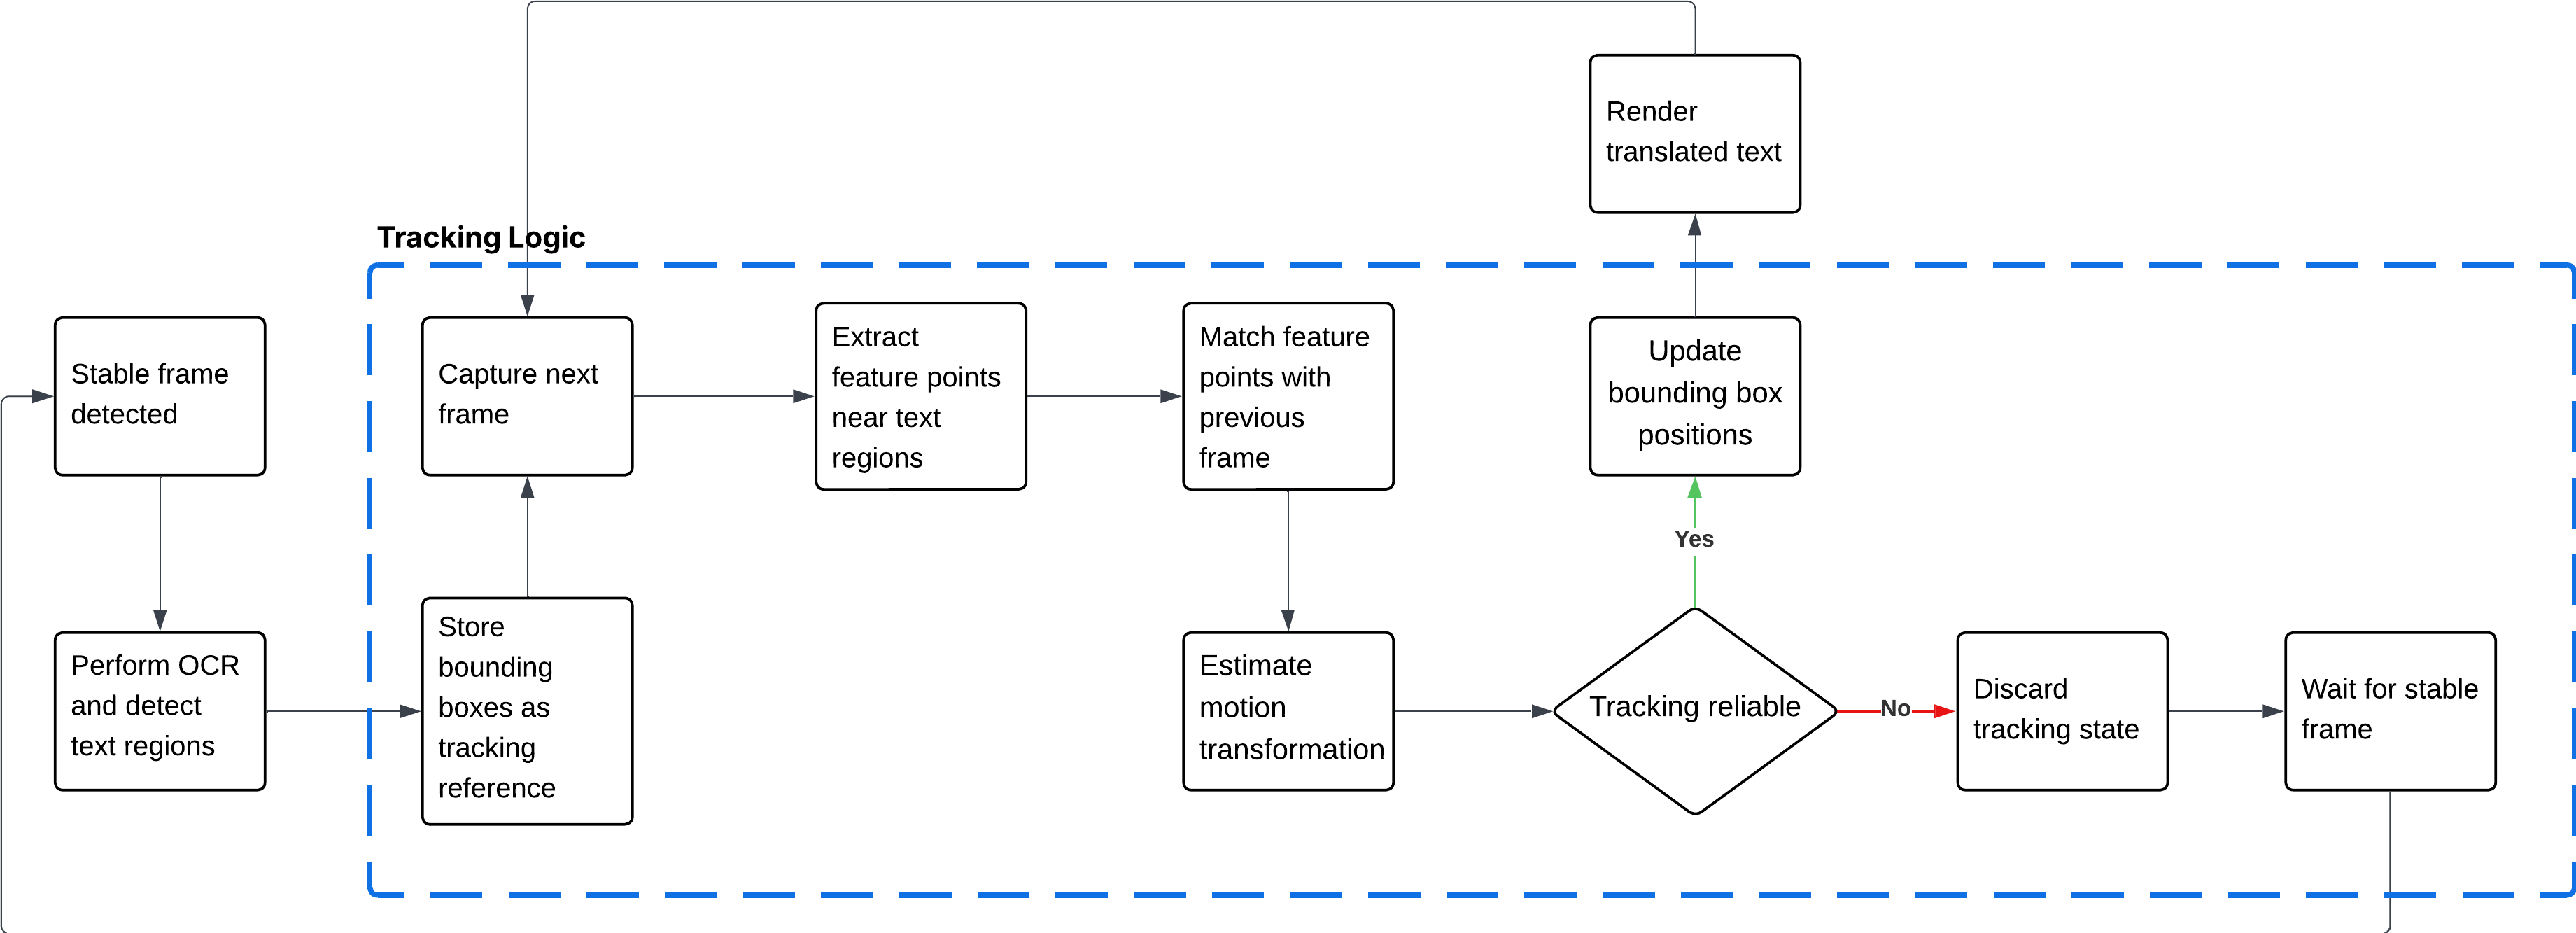
\includegraphics[width=\linewidth]{fig/tracking.png}
    \caption{Implementation of the tracking mechanism}
    \label{fig:textlens-tracking-mechanism}
\end{figure}

\subsection{Asynchronous Frame Processing with Kotlin Coroutines}

To maintain real-time responsiveness, OCR, translation, and image processing tasks are executed asynchronously using \textbf{Kotlin Coroutines}. This is important because the application processes a continuous stream of camera frames, and operations such as text recognition, translation, and scene text replacement are computationally expensive. If these tasks were executed directly on the main UI thread, the application would become unresponsive, causing frame drops, delayed camera preview updates, and poor user experience.

In TextLens, coroutines are used to move heavy processing tasks onto background threads while keeping the main thread free for user interaction and interface updates. When a new frame is captured, the expensive stages of the pipeline---such as OCR, translation, and OpenCV-based image manipulation---can be launched in a background context (for example, using \texttt{Dispatchers.IO} or other worker threads). This allows the system to continue displaying the live camera preview smoothly while the frame is being processed in parallel. 


Once the background processing is complete, the result is safely returned to the main thread for UI rendering. This is necessary because Android UI components must be updated only on the main thread. By separating heavy computation from UI updates, the application can maintain both responsiveness and correctness during continuous operation.

Another advantage of using coroutines is that they support structured and manageable asynchronous execution. Since TextLens operates on a frame-by-frame basis, multiple processing steps must be coordinated without blocking one another. Coroutines make it easier to organize these steps in sequence, handle cancellation when frames become outdated, and prevent the application from wasting resources on unnecessary processing. This is particularly useful in a real-time camera application, where newer frames may arrive before earlier frames have finished processing.

\begin{figure}[H]
    \centering
    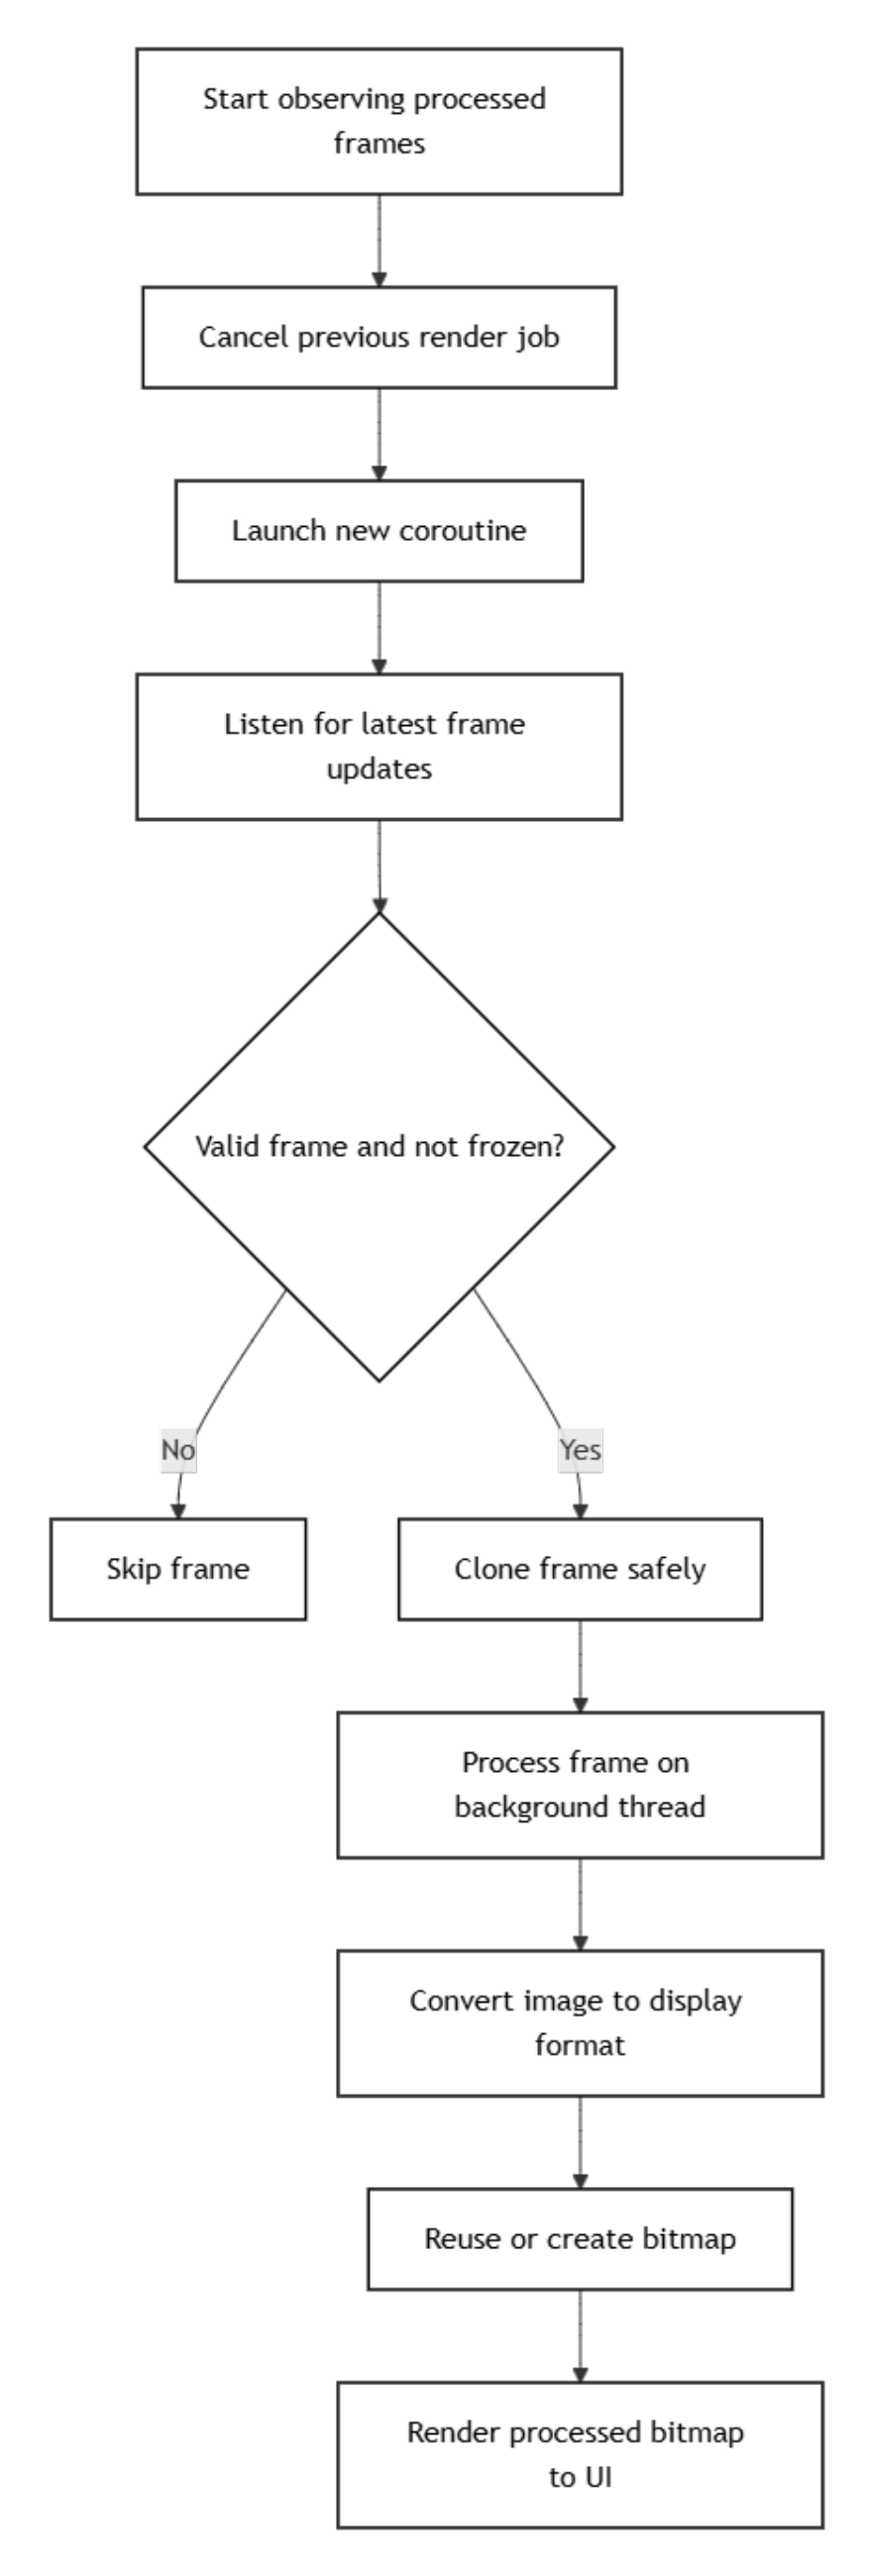
\includegraphics[width=0.5\linewidth]{fig/coroutineflowchart}
    \caption{Data flow using coroutines and asynchronous processing}
    \label{fig:coroutines-flow}
\end{figure}

\section{Offline Capability and On-Device Model Management}

One of the key design goals of TextLens is the ability to operate without continuous Wi-Fi or mobile data connectivity. To achieve this, the system is implemented using on-device machine learning models for both text recognition and translation. Instead of relying on cloud-based APIs, all major processing components execute locally on the Android device once the required language models are installed.

\subsection{On-Device Optical Character Recognition}

Text recognition in TextLens is performed using ML Kit's on-device OCR. The recognizers are initialized directly within the Android application and run entirely on the device. This eliminates the need to upload captured images to a remote server for processing. Since OCR is executed locally, text detection and bounding box extraction continue to function even when the device is offline.

The OCR pipeline processes camera frames captured via CameraX and returns recognized text along with spatial information such as bounding boxes and corner points. Because this step does not require network communication, the application remains responsive and independent of internet connectivity during recognition.

\subsection{On-Device Neural Machine Translation}

Translation is also implemented using ML Kit's on-device neural machine translation models. Unlike cloud-based translation services, the selected language model is downloaded once and stored locally on the device. After installation, translation requests are handled fully offline.

In the program, language model management is explicitly handled before translation begins. The application checks whether the required target language model has already been downloaded. If the model exists, translation proceeds immediately. If not, the system prompts the user to download the model when Wi-Fi is available. Once downloaded, the model remains stored locally and can be reused across sessions.

After the model has been downloaded successfully, the translation process does not require further internet access. This design allows TextLens to continue functioning in environments with poor connectivity, such as rural areas or while travelling.

\subsection{Local Model Persistence Across Sessions}

Downloaded translation models are stored persistently by the ML Kit framework. This means that once a user downloads a language pack, it remains available even after the application is closed and reopened. The program also queries the model manager to determine which language models are already installed, allowing the UI to display available languages without requiring network checks.

By managing language models locally and separating the download phase from the runtime translation phase, the system ensures that:

\begin{itemize}
    \item OCR operates fully offline.
    \item Translation operates offline after initial model installation.
    \item No image data is transmitted externally during normal usage.
    \item The application remains usable in low-connectivity environments.
\end{itemize}

\subsection{Design Trade-Off}

While TextLens supports offline translation, the initial download of a new language model still requires internet access. However, this is a one-time setup cost per language. After installation, all recognition and translation tasks are performed locally, ensuring privacy, reduced latency, and improved reliability.

Overall, the use of on-device OCR and translation models is central to enabling TextLens to function as an offline, real-time mobile scene text translation application.
